\documentclass[nofonts,x11names]{tufte-handout}

% ams
\usepackage{amssymb,amsmath}

\usepackage{ifxetex,ifluatex}
\usepackage{fixltx2e} % provides \textsubscript
\ifnum 0\ifxetex 1\fi\ifluatex 1\fi=0 % if pdftex
  \usepackage[T1]{fontenc}
  \usepackage[utf8]{inputenc}
\else % if luatex or xelatex
  \makeatletter
  \@ifpackageloaded{fontspec}{}{\usepackage{fontspec}}
  \makeatother
  \defaultfontfeatures{Ligatures=TeX,Scale=MatchLowercase}
  \makeatletter
  \@ifpackageloaded{soul}{
     \renewcommand\allcapsspacing[1]{{\addfontfeature{LetterSpace=15}#1}}
     \renewcommand\smallcapsspacing[1]{{\addfontfeature{LetterSpace=10}#1}}
   }{}
  \makeatother
\fi

% graphix
\usepackage{graphicx}
\setkeys{Gin}{width=\linewidth,totalheight=\textheight,keepaspectratio}

% booktabs
\usepackage{booktabs}

% url
\usepackage{url}

% hyperref
\usepackage{hyperref}

% units.
\usepackage{units}


\setcounter{secnumdepth}{2}

% citations
\usepackage{natbib}
\bibliographystyle{plainnat}

%% tint override
\setcitestyle{round} 

% pandoc syntax highlighting

% longtable

% multiplecol
\usepackage{multicol}

% strikeout
\usepackage[normalem]{ulem}

% morefloats
\usepackage{morefloats}


% tightlist macro required by pandoc >= 1.14
\providecommand{\tightlist}{%
  \setlength{\itemsep}{0pt}\setlength{\parskip}{0pt}}

% title / author / date
\title{P3: CarbFix:}
\author{ETT}
\date{2025-02-16}

%% -- tint overrides
%% fonts, using roboto (condensed) as default
\usepackage[sfdefault,condensed]{roboto}
%% also nice: \usepackage[default]{lato}

%% colored links, setting 'borrowed' from RJournal.sty with 'Thanks, Achim!'
\RequirePackage{color}
\definecolor{link}{rgb}{0.1,0.1,0.8} %% blue with some grey
\hypersetup{
  colorlinks,%
  citecolor=link,%
  filecolor=link,%
  linkcolor=link,%
  urlcolor=link
}

%% macros
\makeatletter

%% -- tint does not use italics or allcaps in title
\renewcommand{\maketitle}{%     
  \newpage
  \global\@topnum\z@% prevent floats from being placed at the top of the page
  \begingroup
    \setlength{\parindent}{0pt}%
    \setlength{\parskip}{4pt}%
    \let\@@title\@empty
    \let\@@author\@empty
    \let\@@date\@empty
    \ifthenelse{\boolean{@tufte@sfsidenotes}}{%
      %\gdef\@@title{\sffamily\LARGE\allcaps{\@title}\par}%
      %\gdef\@@author{\sffamily\Large\allcaps{\@author}\par}%
      %\gdef\@@date{\sffamily\Large\allcaps{\@date}\par}%
      \gdef\@@title{\begingroup\fontseries{b}\selectfont\LARGE{\@title}\par}%
      \gdef\@@author{\begingroup\fontseries{l}\selectfont\Large{\@author}\par}%
      \gdef\@@date{\begingroup\fontseries{l}\selectfont\Large{\@date}\par}%
    }{%
      %\gdef\@@title{\LARGE\itshape\@title\par}%
      %\gdef\@@author{\Large\itshape\@author\par}%
      %\gdef\@@date{\Large\itshape\@date\par}%
      \gdef\@@title{\begingroup\fontseries{b}\selectfont\LARGE\@title\par\endgroup}%
      \gdef\@@author{\begingroup\fontseries{l}\selectfont\Large\@author\par\endgroup}%
      \gdef\@@date{\begingroup\fontseries{l}\selectfont\Large\@date\par\endgroup}%
    }%
    \@@title
    \@@author
    \@@date
  \endgroup
  \thispagestyle{plain}% suppress the running head
  \tuftebreak% add some space before the text begins
  \@afterindentfalse\@afterheading% suppress indentation of the next paragraph
}

%% -- tint does not use italics or allcaps in section/subsection/paragraph
\titleformat{\section}%
  [hang]% shape
  %{\normalfont\Large\itshape}% format applied to label+text
  {\fontseries{b}\selectfont\Large}% format applied to label+text
  {\thesection}% label
  {1em}% horizontal separation between label and title body
  {}% before the title body
  []% after the title body

\titleformat{\subsection}%
  [hang]% shape
  %{\normalfont\large\itshape}% format applied to label+text
  {\fontseries{m}\selectfont\large}% format applied to label+text
  {\thesubsection}% label
  {1em}% horizontal separation between label and title body
  {}% before the title body
  []% after the title body

\titleformat{\paragraph}%
  [runin]% shape
  %{\normalfont\itshape}% format applied to label+text
  {\fontseries{l}\selectfont}% format applied to label+text
  {\theparagraph}% label
  {1em}% horizontal separation between label and title body
  {}% before the title body
  []% after the title body

%% -- tint does not use italics here either
% Formatting for main TOC (printed in front matter)
% {section} [left] {above} {before w/label} {before w/o label} {filler + page} [after]
\ifthenelse{\boolean{@tufte@toc}}{%
  \titlecontents{part}% FIXME
    [0em] % distance from left margin
    %{\vspace{1.5\baselineskip}\begin{fullwidth}\LARGE\rmfamily\itshape} % above (global formatting of entry)
    {\vspace{1.5\baselineskip}\begin{fullwidth}\fontseries{m}\selectfont\LARGE} % above (global formatting of entry)
    {\contentslabel{2em}} % before w/label (label = ``II'')
    {} % before w/o label
    {\rmfamily\upshape\qquad\thecontentspage} % filler + page (leaders and page num)
    [\end{fullwidth}] % after
  \titlecontents{chapter}%
    [0em] % distance from left margin
    %{\vspace{1.5\baselineskip}\begin{fullwidth}\LARGE\rmfamily\itshape} % above (global formatting of entry)
    {\vspace{1.5\baselineskip}\begin{fullwidth}\fontseries{m}\selectfont\LARGE} % above (global formatting of entry)
    {\hspace*{0em}\contentslabel{2em}} % before w/label (label = ``2'')
    {\hspace*{0em}} % before w/o label
    %{\rmfamily\upshape\qquad\thecontentspage} % filler + page (leaders and page num)
    {\upshape\qquad\thecontentspage} % filler + page (leaders and page num)
    [\end{fullwidth}] % after
  \titlecontents{section}% FIXME
    [0em] % distance from left margin
    %{\vspace{0\baselineskip}\begin{fullwidth}\Large\rmfamily\itshape} % above (global formatting of entry)
    {\vspace{0\baselineskip}\begin{fullwidth}\fontseries{m}\selectfont\Large} % above (global formatting of entry)
    {\hspace*{2em}\contentslabel{2em}} % before w/label (label = ``2.6'')
    {\hspace*{2em}} % before w/o label
    %{\rmfamily\upshape\qquad\thecontentspage} % filler + page (leaders and page num)
    {\upshape\qquad\thecontentspage} % filler + page (leaders and page num)
    [\end{fullwidth}] % after
  \titlecontents{subsection}% FIXME
    [0em] % distance from left margin
    %{\vspace{0\baselineskip}\begin{fullwidth}\large\rmfamily\itshape} % above (global formatting of entry)
    {\vspace{0\baselineskip}\begin{fullwidth}\fontseries{m}\selectfont\large} % above (global formatting of entry)
    {\hspace*{4em}\contentslabel{4em}} % before w/label (label = ``2.6.1'')
    {\hspace*{4em}} % before w/o label
    %{\rmfamily\upshape\qquad\thecontentspage} % filler + page (leaders and page num)
    {\upshape\qquad\thecontentspage} % filler + page (leaders and page num)
    [\end{fullwidth}] % after
  \titlecontents{paragraph}% FIXME
    [0em] % distance from left margin
    %{\vspace{0\baselineskip}\begin{fullwidth}\normalsize\rmfamily\itshape} % above (global formatting of entry)
    {\vspace{0\baselineskip}\begin{fullwidth}\fontseries{m}\selectfont\normalsize\rmfamily} % above (global formatting of entry)
    {\hspace*{6em}\contentslabel{2em}} % before w/label (label = ``2.6.0.0.1'')
    {\hspace*{6em}} % before w/o label
    %{\rmfamily\upshape\qquad\thecontentspage} % filler + page (leaders and page num)
    {\upshape\qquad\thecontentspage} % filler + page (leaders and page num)
    [\end{fullwidth}] % after
}{}

  
\makeatother


\usepackage{mhchem}

\begin{document}

\maketitle




\newcommand{\mathalert}[1]{\textcolor{red}{\mathbf{#1}}}

\newcommand{\highlight}[2][yellow]{\mathchoice%
  {\colorbox{#1}{$\displaystyle#2$}}%
  {\colorbox{#1}{$\textstyle#2$}}%
  {\colorbox{#1}{$\scriptstyle#2$}}%
  {\colorbox{#1}{$\scriptscriptstyle#2$}}}

\newcommand{\carb}{CO$_2$}
\newcommand{\dC}{$\delta$$^{13}$C}
\newcommand{\micmoll}{$\mu$mol/l}
\newcommand{\bicarb}{$HCO_{3}^-$}
\newcommand{\sulfate}{SO$_4^{2-}$}

\colorlet{very-short-term}{LightPink1}
\colorlet{short-term}{LightBlue1}
\colorlet{long-term}{LightGoldenrod1}

\marginnote{This is an R markdown document.  It is similar to a jupyter notebook that you might be more familiar with.  You can both explore the code, and also compile the final document to pdf output.  This should provide you with some familiarisation of "R", as well as the science.}

This practical will take place on your laptops via a web-browser
(hopefully). Navigate to moodle in a web browser and click on the link
to the CarFix practical. This will open a Binder webpage which will
compile into an interface that is identical to the RStudio App. Some of
you will be familiar with this app, but if you have never used if before
you will. need to spend a few minutes familiarising yourself with it and
making sure you know how to run R.

\noindent The
CarbFix\marginnote{Those of you who took petrology at PII may well have heard about CarbFix already.}
project in Iceland was created to develop the technology to store carbon
dioxide as stable carbonate minerals directly in the subsurface by
reacting gas charged injection waters with basaltic rocks. Carbon
storage in basaltic rocks offers numerous advantages including their
ability to promote mineral carbonation and their large potential storage
volume. Numerous studies have focused on developing the technology to
safely store \carb~in basaltic rocks including laboratory experiments,
modelling and field studies. Basaltic rocks are rich in divalent cations
such as \ce{Ca^{2+}}, \ce{Mg^{2+}}, and \ce{Fe^{2+}}. The injection of
acidic water enriched in \ce{CO2} promotes the release of these
cations\marginnote{\ce{Fe^{2+}} is not a typical cation in natural waters.  Think about why it is a cation in these particular waters},
potentially leading to the formation of carbonate minerals such as
calcite, magnesite, and siderite as the continued dissolution of basalt
increases the pH of the aqueous fluid. About 5\% of the continents and
most of the oceanic floor are comprised of basaltic rocks, including the
mid-oceanic ridges. As such the largest basaltic storage potential lies
offshore; theoretically all \ce{CO2} from the burning of fossil fuel
carbon (estimated to be ca.
5000Gt)\marginnote{Do you remember how much carbon is in the ocean-atmosphere system?}.
The flanks of mid-ocean ridges contain highly fractured and permeable
basaltic layers with a pervasive hydrothermal circulation of about
1000Gt seawater/yr. Lab results have demonstrated that basaltic rocks
dissolve rapidly in seawater which is rich in \carb.
\marginnote{Note that there has already been a sequel to CarbFix, CarbFix2, which now has a sequel "Seastone"}

The CarbFix injection site is equipped with a 2000m deep injection well
and 8 monitoring wells ranging in depth from 50 to 1300m in depth. The
subsurface rocks at the injection site are primarily olivine tholeiite
basalts consisting of lava flows and hyaloclastite formations. The
hyaloclastites are relatively low permeability glassy rocks formed under
ice and melt water during glaciations; the boundaries between
hyaloclastites and lava flows, and those between individual lava flows
boundaries are preferential fluid flow pathways. Some alteration is
observed in the hyaloclastite rocks starting at 120--300m depth. The
common alteration minerals at this depth are smectite, calcite, Ca-rich
zeolites, and poorly crystalline iron-hydroxides.

Fluid injection was targeted at a lava flow sequence located 400--800m
below the surface with the main aquifer located at ca.530m depth. Loss
on ignition measurements on rock samples suggest that over 80\% of the
primary rocks in the target zone are currently unaltered. Tracer tests
were conducted both under natural and forced flow conditions from 2008
to 2011 to define the system hydrology. These tests indicated that the
flow from the HN-02 injection well to the first monitoring well (HN-04)
consists of relatively homogenous porous media intersected by a low
volume and fast flow path that channels about 3\% of the tracer flow.

\begin{figure*}

{\centering 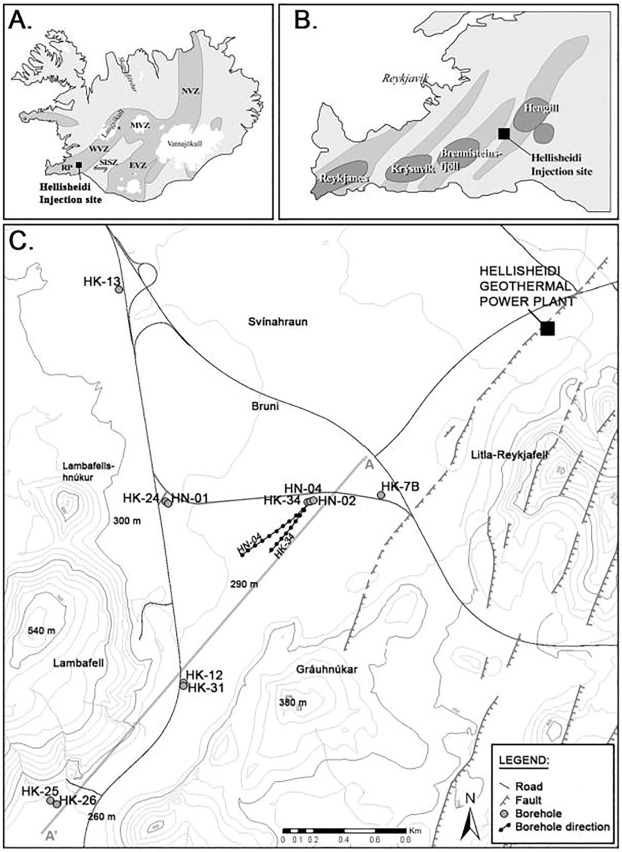
\includegraphics[width=0.8\linewidth]{Figs/Carbfix_map} 

}

\caption[Map of the Carbfix site from @OELKERS2018]{Map of the Carbfix site from @OELKERS2018}\label{fig:unnamed-chunk-1}
\end{figure*}

\begin{figure*}

{\centering 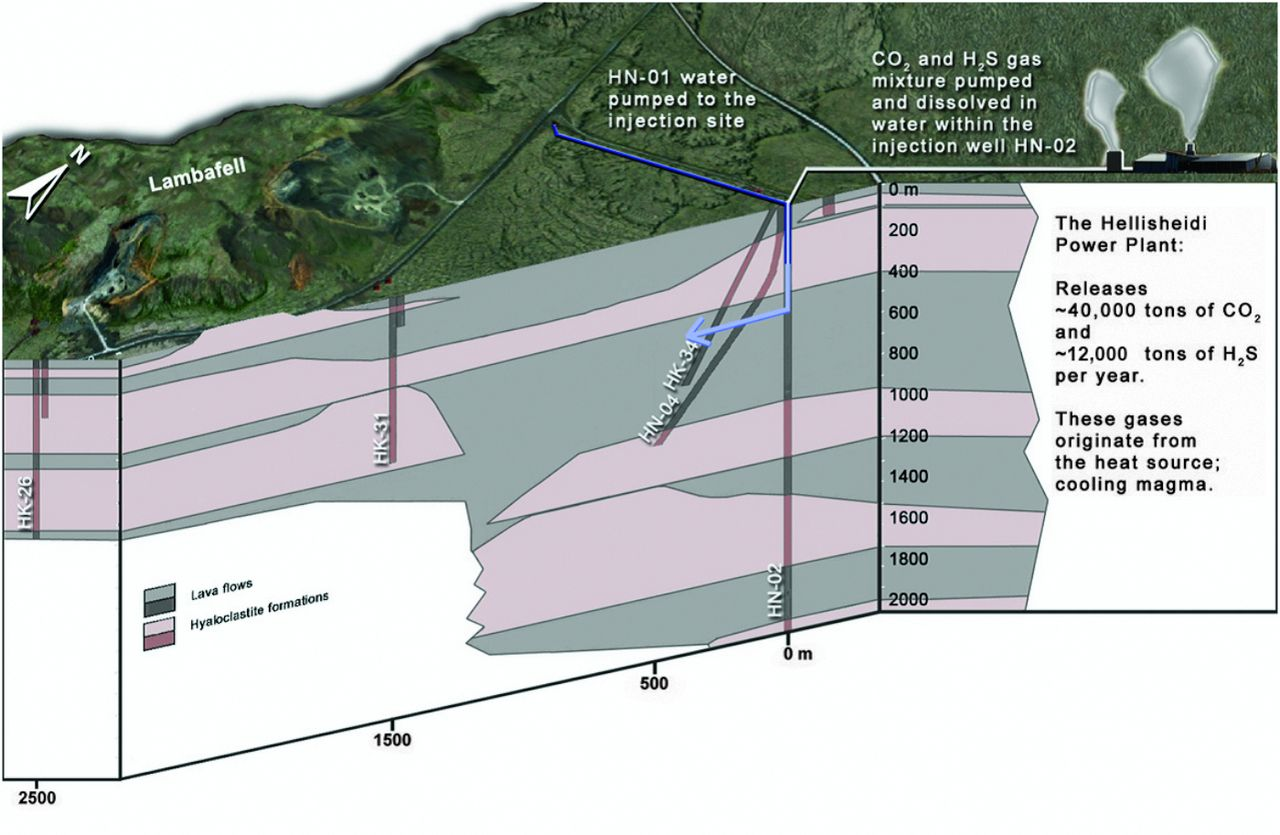
\includegraphics[width=0.8\linewidth]{Figs/CarbFix_section} 

}

\caption[Section of the Carbfix site from @Matter:2016aa]{Section of the Carbfix site from @Matter:2016aa}\label{fig:unnamed-chunk-2}
\end{figure*}

\carb~was injected dissolved in seawater in two phases (phase I and
phase II). The injection fluid was spiked with nonreactive but volatile
sulfur hexafluoride (\ce{SF6}) and trifluoromethyl sulfur pentafluoride
(\ce{SF5CF3}) tracers to assess plume migration in the reservoir. The
\ce{SF6} was used during phase I and \ce{SF5CF3} during phase II.

Because dissolved or mineralized \ce{CO2} cannot be detected by
conventional monitoring methods such as seismic imaging, the fate of the
injected \ce{CO2} was monitored with a suite of chemical and isotopic
tracers. The injected \ce{CO2} was spiked with carbon-14 (\ce{14C}) to
monitor its transport and reactivity.

\section{\texorpdfstring{TASK: Read in the data from
\citet{Matter:2016aa}.}{TASK: Read in the data from @Matter:2016aa.}}\label{task-read-in-the-data-from-matter2016aa.}

\noindent Note that this data was collected from in monitoring well
HN04.

\section{\texorpdfstring{TASK: Plot a graph of \ce{SF_6} and
\ce{SF5CF3}versus days after
injection.}{TASK: Plot a graph of  and versus days after injection.}}\label{task-plot-a-graph-of-and-versus-days-after-injection.}

\begin{figure*}
\includegraphics{Carbfix_files/figure-latex/SF6 time carbfix-1} \caption[SF6 vs days after injection]{SF6 vs days after injection.  Blue shaded areas correspond to injection periods.}\label{fig:SF6 time carbfix}
\end{figure*}

\section{\texorpdfstring{QUESTION: Noting that the \ce{SF6} and
\ce{SF5CF3} are inert tracers, suggest when the injected \carb~rich
fluid was detected at the HN04 monitoring
well.}{QUESTION: Noting that the  and  are inert tracers, suggest when the injected ~rich fluid was detected at the HN04 monitoring well.}}\label{question-noting-that-the-and-are-inert-tracers-suggest-when-the-injected-rich-fluid-was-detected-at-the-hn04-monitoring-well.}

\section{TASK: Plot a graph of 14C versus days after
injection.}\label{task-plot-a-graph-of-14c-versus-days-after-injection.}

\begin{marginfigure}[0.5cm]
\includegraphics{Carbfix_files/figure-latex/14C time carbfix-1} \caption[14C vs days after injection]{14C vs days after injection.  Blue shaded areas correspond to injection periods.}\label{fig:14C time carbfix}
\end{marginfigure}

\noindent The 14C concentrations of the injected fluids were 40.0
Bq/liter and 6 Bq/liter, respectively. By comparison, the 14C
concentration in the reservoir before the injections was 0.0006
Bq/liter.

\section{QUESTION: How long does the fluid take to break though at the
monitoring well
HN04?}\label{question-how-long-does-the-fluid-take-to-break-though-at-the-monitoring-well-hn04}

\section{QUESTION: What happens to 14C at the monitoring well during the
injection period? Suggest possible
explanations.}\label{question-what-happens-to-14c-at-the-monitoring-well-during-the-injection-period-suggest-possible-explanations.}

\section{TASK: Plot a graph of pH versus days after
injection.}\label{task-plot-a-graph-of-ph-versus-days-after-injection.}

\begin{marginfigure}[0.5cm]
\includegraphics{Carbfix_files/figure-latex/pH time carbfix-1} \caption[pH vs days after injection]{pH vs days after injection.  Blue shaded areas correspond to injection periods.}\label{fig:pH time carbfix}
\end{marginfigure}

\section{QUESTION: What happens to the pH at the monitoring well during
the injection period?
Why?}\label{question-what-happens-to-the-ph-at-the-monitoring-well-during-the-injection-period-why}

\clearpage

\section{TASK: Plot a graph of DIC versus days after
injection.}\label{task-plot-a-graph-of-dic-versus-days-after-injection.}

\begin{marginfigure}[-0.55cm]
\includegraphics{Carbfix_files/figure-latex/DIC time carbfix-1} \caption[DIC vs days after injection]{DIC vs days after injection.  Blue shaded areas correspond to injection periods.}\label{fig:DIC time carbfix}
\end{marginfigure}

\section{QUESTION: What happens to DIC at the monitoring well during the
injection period? Suggest possible
explanations.}\label{question-what-happens-to-dic-at-the-monitoring-well-during-the-injection-period-suggest-possible-explanations.}

The fate of the injected \ce{CO2} was quantified using mass balance
calculations. The mixing fraction between the injected solution (\(IS\))
and ambient groundwater (\(GW\)) was calculated for each extracted water
sample (i) using: \begin{equation}
[SF_6]_i=X[SF_6]_{IS}+(1-X)[SF_6]_{GW}
\end{equation}\marginnote{This kind of simple mass balance equation should be familiar to you and you should expect to know how to formulate and use it.}
with \(X\) being the fraction of injected solution in the extracted
water sample

\section{\texorpdfstring{TASK: Compute the mixing fraction X for each of
the samples in the \citet{Matter:2016aa} dataset. Note that the \ce{SF6}
and \ce{SF5CF3} concentrations in the injected fluids were
\(2.33 \times 10^{-8} cc\) at standard temperature and pressure
(ccSTP)/cc and \(2.24 \times 10^{-8}\) ccSTP/cc, respectively. Assume
that the concentrations of \ce{SF6} and \ce{SF5CF3} in ambient
groundwater are
zero.}{TASK: Compute the mixing fraction X for each of the samples in the @Matter:2016aa dataset. Note that the  and  concentrations in the injected fluids were 2.33 \textbackslash times 10\^{}\{-8\} cc at standard temperature and pressure (ccSTP)/cc and 2.24 \textbackslash times 10\^{}\{-8\} ccSTP/cc, respectively. Assume that the concentrations of  and  in ambient groundwater are zero.}}\label{task-compute-the-mixing-fraction-x-for-each-of-the-samples-in-the-matter2016aa-dataset.-note-that-the-and-concentrations-in-the-injected-fluids-were-2.33-times-10-8-cc-at-standard-temperature-and-pressure-ccstpcc-and-2.24-times-10-8-ccstpcc-respectively.-assume-that-the-concentrations-of-and-in-ambient-groundwater-are-zero.}

\noindent The expected DIC values due to pure mixing between the
injected fluid and ambient groundwater can be determined from:
\begin{equation}
DIC_{mix}=X[DIC]_{IS}+(1-X)DIC_{GW}
\end{equation} This is the DIC that would be expected assuming
conservative mixing based on the \ce{SF_6} data. The alkalinity of the
groundwater from monitoring well HN-4 was 1.91meq/L and the pH was 9.43
at 20C. Remember that alkalinity is not the same as DIC, but DIC can be
calculated from the alkalinity given the pH.

\section{TASK Determine the DIC of the ambient
groundwater.}\label{task-determine-the-dic-of-the-ambient-groundwater.}

\marginnote[-2cm]{If you are not clear about how to calculate the DIC, it will make an ideal supervision exercise......}

\section{\texorpdfstring{TASK: Compute the \(DIC_{mix}\) assuming the
conservative behaviour of \ce{SF6}. Note that the \(\sf DIC_{IS}\) was
0.82 mol/liter in phase 1. Note that this assumes that DIC has behaved
conservatively.}{TASK: Compute the DIC\_\{mix\} assuming the conservative behaviour of . Note that the \textbackslash sf DIC\_\{IS\} was 0.82 mol/liter in phase 1. Note that this assumes that DIC has behaved conservatively.}}\label{task-compute-the-dic_mix-assuming-the-conservative-behaviour-of-.-note-that-the-sf-dic_is-was-0.82-molliter-in-phase-1.-note-that-this-assumes-that-dic-has-behaved-conservatively.}

\marginnote[-1.4cm]{Note that as calculated here it is greatly exaggerating the effect in the @Matter:2016aa paper.  The conclusion is similar, but exaggerated.  On reading the @Matter:2016aa paper I've not managed to understand why the calculations are not reproducing their numbers.}

\section{\texorpdfstring{TASK: Plot the \(DIC_{mix}\) and DIC on the
same graph. What do you notice about the difference between
\(DIC_{mix}\) and the measured DIC? What do you infer has
happened?}{TASK: Plot the DIC\_\{mix\} and DIC on the same graph. What do you notice about the difference between DIC\_\{mix\} and the measured DIC? What do you infer has happened?}}\label{task-plot-the-dic_mix-and-dic-on-the-same-graph.-what-do-you-notice-about-the-difference-between-dic_mix-and-the-measured-dic-what-do-you-infer-has-happened}

\begin{marginfigure}[0.1cm]
\includegraphics{Carbfix_files/figure-latex/DIC time carbfix, with DIC_mix-1} \caption[DIC vs days after injection]{DIC vs days after injection. Red data is modelled. Blue shaded areas correspond to injection periods.}\label{fig:DIC time carbfix, with DIC_mix}
\end{marginfigure}

\noindent The expected \(\sf ^{14}C\) values due to pure mixing between
the injected fluid and ambient groundwater can be determined from:
\begin{equation}
^{14}C_{mix}=X^{14}C_{IS}+(1-X)^{14}C_{GW}
\end{equation}

\section{\texorpdfstring{TASK: Compute the \(\sf ^{14}C_{mix}\) assuming
the conservative behaviour of \ce{SF6}. Note that the
\(\sf ^{14}C_{IS}\) was 40.0 Bq/liter in phase 1. By comparison, the
\(^{14}C\) concentration in the reservoir before the injections
(\(\sf ^{14}C_{GW}\)) was 0.0006 Bq/liter. Note that this assumes that
DIC has behaved
conservatively.}{TASK: Compute the \textbackslash sf \^{}\{14\}C\_\{mix\} assuming the conservative behaviour of . Note that the \textbackslash sf \^{}\{14\}C\_\{IS\} was 40.0 Bq/liter in phase 1. By comparison, the \^{}\{14\}C concentration in the reservoir before the injections (\textbackslash sf \^{}\{14\}C\_\{GW\}) was 0.0006 Bq/liter. Note that this assumes that DIC has behaved conservatively.}}\label{task-compute-the-sf-14c_mix-assuming-the-conservative-behaviour-of-.-note-that-the-sf-14c_is-was-40.0-bqliter-in-phase-1.-by-comparison-the-14c-concentration-in-the-reservoir-before-the-injections-sf-14c_gw-was-0.0006-bqliter.-note-that-this-assumes-that-dic-has-behaved-conservatively.}

\section{\texorpdfstring{TASK: Plot the \(\sf ^{14}C_{mix}\) and
\(\sf ^{14}C\) on the same graph. What do you notice about the
difference between \(\sf ^{14}C_{mix}\) and the measured \(\sf ^{14}C\)?
What do you infer has
happened?}{TASK: Plot the \textbackslash sf \^{}\{14\}C\_\{mix\} and \textbackslash sf \^{}\{14\}C on the same graph. What do you notice about the difference between \textbackslash sf \^{}\{14\}C\_\{mix\} and the measured \textbackslash sf \^{}\{14\}C? What do you infer has happened?}}\label{task-plot-the-sf-14c_mix-and-sf-14c-on-the-same-graph.-what-do-you-notice-about-the-difference-between-sf-14c_mix-and-the-measured-sf-14c-what-do-you-infer-has-happened}

\begin{marginfigure}[-2cm]
\includegraphics{Carbfix_files/figure-latex/14C time carbfix, with DIC_mix-1} \caption[DIC vs days after injection]{DIC vs days after injection.  Blue shaded areas correspond to injection periods.}\label{fig:14C time carbfix, with DIC_mix}
\end{marginfigure}

\noindent Differences in DIC and 14C concentrations between the values
measured in the retrieved fluid samples and the expected values assuming
only mixing between injectate and ambient groundwater yield the loss of
DIC and 14C due to carbonate precipitation.

\section{TASK: Use the lever rule to estimate the loss of DIC, compared
to conservative behaviour defined by mixing between injection waters and
ambient
groundwater.}\label{task-use-the-lever-rule-to-estimate-the-loss-of-dic-compared-to-conservative-behaviour-defined-by-mixing-between-injection-waters-and-ambient-groundwater.}

\section{TASK: Plot a graph of the fraction of DIC
loss.}\label{task-plot-a-graph-of-the-fraction-of-dic-loss.}

\begin{marginfigure}[-1cm]
\includegraphics{Carbfix_files/figure-latex/DIC fractional loss time carbfix-1} \caption[DIC vs days after injection]{DIC vs days after injection.  Blue shaded areas correspond to injection periods.}\label{fig:DIC fractional loss time carbfix}
\end{marginfigure}

The fast conversion rate of dissolved \ce{CO2} to calcite minerals in
the CarbFix storage reservoir is most likely the result of several key
processes:

\begin{enumerate}
\item The novel \ce{CO2} injection system that injected water-dissolved \ce{CO2} into the subsurface
\item The relatively rapid dissolution rate of basalt, releasing Ca, Mg, and Fe ions required for the \ce{CO2} mineralization,
\item The mixing of injected water with alkaline formation waters,
\item The dissolution of preexisting secondary carbonates at the onset of the \ce{CO2} injection, which may have contributed to the neutralization of the injected \ce{CO2}-rich water via the reaction $\sf CaCO_3 + CO_2 + H_2O = Ca^{2+} + 2 HCO3^-$.
\end{enumerate}

\noindent The efficiency of mineral carbonation, however, can be limited
if Mg clay minerals rather than Mg carbonate minerals form in response
to the injection of \ce{CO2} into basalts. Magnesium clay formation is
detrimental to carbon storage efforts because these minerals consume
divalent Mg that could otherwise be used for carbonate mineral
formation, and because Mg-bearing clays could decrease host rock
permeability. Mg has three stable isotopes (\(^{24}Mg\), \(^{25}Mg\) and
\(^{26}Mg\)) which are thought to be fractionated by the formation of
clay minerals \citet{Hindshaw:2020aa}.

\noindent Will Knapp and ETT have been compiling a database of Mg
isotope data that has been published to date.

\section{TASK: Read in a Mg isotope database of all data to
date.}\label{task-read-in-a-mg-isotope-database-of-all-data-to-date.}

\section{TASK: Make a plot of the evolution of the number of published
Mg isotope data over the last
decade.}\label{task-make-a-plot-of-the-evolution-of-the-number-of-published-mg-isotope-data-over-the-last-decade.}

\begin{figure}
\includegraphics{Carbfix_files/figure-latex/Mg isotope publications plot-1} \caption[Summary of how much Mg isotope data has been published to date]{Summary of how much Mg isotope data has been published to date}\label{fig:Mg isotope publications plot}
\end{figure}

\noindent The data has been categorised for you so that global trends in
the data can be teased out.

\section{TASK: Run the following chunk to tidy up these
categories.}\label{task-run-the-following-chunk-to-tidy-up-these-categories.}

\section{TASK: Run the following script that makes a plot summarising
the whole
database.}\label{task-run-the-following-script-that-makes-a-plot-summarising-the-whole-database.}

\marginnote{The "dots" at the end of the boxplot represent outliers. There are a number of different rules for determining if a point is an outlier, but the method that R and ggplot use is the "1.5 rule". Outliers are defined by:  
\begin{enumerate}
\item less than $Q1 - 1.5*IQR$
\item greater than $Q3 + 1.5*IQR$
\end{enumerate}
Where Q refers to a quartile.
The whiskers are defined as:
\begin{enumerate}
\item $upper whisker = min(max(x), Q_3 + 1.5 * IQR)$
\item $lower whisker = max(min(x), Q_1 – 1.5 * IQR)$
\end{enumerate}
The box is defined by the interquartile range ($IQR = Q_3 – Q_1$) 
}

\begin{figure}
\includegraphics{Carbfix_files/figure-latex/Mg caltech plot-1} \caption[Caltech Mg isotope data published to date]{Caltech Mg isotope data published to date. Red data are outliers.}\label{fig:Mg caltech plot}
\end{figure}

\section{QUESTION: Which of the data categories on the plot suggest that
clay might fractionate Mg
isotopes?}\label{question-which-of-the-data-categories-on-the-plot-suggest-that-clay-might-fractionate-mg-isotopes}

\noindent If you are interested in this you can read more in
\citet{Tipper:2022aa}

\section{QUESTION: What do you note about the range of Silicate rock?
(Hint: Look at the
box).}\label{question-what-do-you-note-about-the-range-of-silicate-rock-hint-look-at-the-box.}

\noindent  Mg isotope ratios have been measured on the fluids from the
monitoring well \citet{OELKERS2018}. \# TASK: Read in the data from
\citet{OELKERS2018}

\section{\texorpdfstring{TASK: Make a graph of \(\sf \delta^{26}Mg\)
versus
time.}{TASK: Make a graph of \textbackslash sf \textbackslash delta\^{}\{26\}Mg versus time.}}\label{task-make-a-graph-of-sf-delta26mg-versus-time.}

\begin{marginfigure}[1cm]
\includegraphics{Carbfix_files/figure-latex/d26Mg carbfix-1} \caption[d26Mg vs date after injection (note the longer period of monitoring)]{d26Mg vs date after injection (note the longer period of monitoring).  Blue shaded areas correspond to injection periods.}\label{fig:d26Mg carbfix}
\end{marginfigure}

\renewcommand\refname{QUESTIONS: By comparing the Mg isotope dta from
Carbfix, with the global compilation of Mg isotope whot do you infer is
happening. Consider 1) What controlled the \(\sf \delta^{26}Mg\) prior
to injection. How doe the \(\sf \delta^{26}Mg\) values compare to the
composition of basalt and seawater? Do the data reflect the
precipitation of carbonate minerals? Do the data reflect the
precipitation of clay minerals?}
\bibliography{Carbfix.bib}



\end{document}
